%%%%%%%%%%%%%%%%%%%%%%%%%%%%%%%%%%%%%%%%%
% CLASS OPTIONS
% language: czech/english/slovak
% thesis type: bachelor/master/dissertation
% color: bw for black&white OR no option for default color scheme
% electronic (oneside) or printed (twoside), twoside is default
% paragraph - if passed, this optional argument sets paragraphs as the deepest level of headers, styles it, numbers it and adds it to Table of Content. Use with care! Normally, it is considered unwise to use it, since its too deep.
%%%%%%%%%%%%%%%%%%%%%%%%%%%%%%%%%%%%%%%%%
\documentclass[english,bachelor,unicode,oneside]{ctufit-thesis}

\ctufittitle{Project adaptation in code completion via in-context learning}
\ctufitauthorfull{Maksim Sapronov}
\ctufitauthorsurnames{Sapronov}
\ctufitauthorgivennames{Maksim}
\ctufitsupervisor{Evgenii Glukhov\, M.Sc.}
\ctufitdepartment{Department of Applied Mathematics}
\ctufityear{2025}
% TODO: understand what declaration is stated about (2 following lines)
\ctufitdeclarationplace{Prague} % replace with the place where you sign the declaration
\ctufitdeclarationdate{\today} % replace with the date of signature of the declaration
% TODO: determine the order of abstracts and fill them in (2 following lines)
\ctufitabstractCZE{Fill in the abstract of this thesis in Czech.}
\ctufitabstractENG{Fill in the abstract of this thesis in English.}
% TODO: determine the order of keywords and fill them in (2 following lines)
\ctufitkeywordsCZE{enter, comma, separated, list, of, keywords, in, CZECH}
\ctufitkeywordsENG{enter, comma, separated, list, of, keywords, in, ENGLISH}

%%%%%%%%%%%%%%%%%%%%%%%%%%%%%%%%%%
% CUSTOMIZATION of this template
% Skip this part or alter it if you know what you are doing.
%%%%%%%%%%%%%%%%%%%%%%%%%%%%%%%%%%

\RequirePackage{iftex}[2020/03/06]
\iftutex % XeLaTeX and LuaLaTeX
    \RequirePackage{ellipsis}[2020/05/22] %ellipsis workaround for XeLaTeX
\else
    \errmessage{Only compilation with XeLaTeX or LuaLaTeX is allowed}
    \stop
\fi

% hyperlinks
\hypersetup{
    pdfpagelayout=TwoPageRight,
    colorlinks=false,
    allcolors=decoration,
    pdfborder={0 0 0.1}
}

% uncomment the following to hide all hyperlinks
%\hypersetup{hidelinks}

% uncomment the following to change the color of all hyperlinks to CTU blue
%\hypersetup{allbordercolors=decoration}

\RequirePackage{pdfpages}[2020/01/28]

%%%%%%%%%%%%%%%%%%%%%%%%%%%%%%%%%%
% CUSTOMIZATION of this template END
%%%%%%%%%%%%%%%%%%%%%%%%%%%%%%%%%%


%%%%%%%%%%%%%%%%%%%%%%
% DEMO CONTENTS SETTINGS
% You may choose to modify this part.
%%%%%%%%%%%%%%%%%%%%%%
\usepackage{dirtree}
\usepackage{lipsum,tikz}
\usepackage[style=authoryear,backend=biber]{biblatex}
\addbibresource{text/bib-database.bib}
\usepackage{xurl}
\usepackage{listings} % typesetting of sources
%\usepackage{minted}
\usepackage{csquotes}

%%%%%%%%%%%%%%%%%%%%%%
% DEMO CONTENTS SETTINGS END
%%%%%%%%%%%%%%%%%%%%%%

\begin{document} 
\frontmatter\frontmatterinit

\thispagestyle{empty}\maketitle\thispagestyle{empty}\cleardoublepage

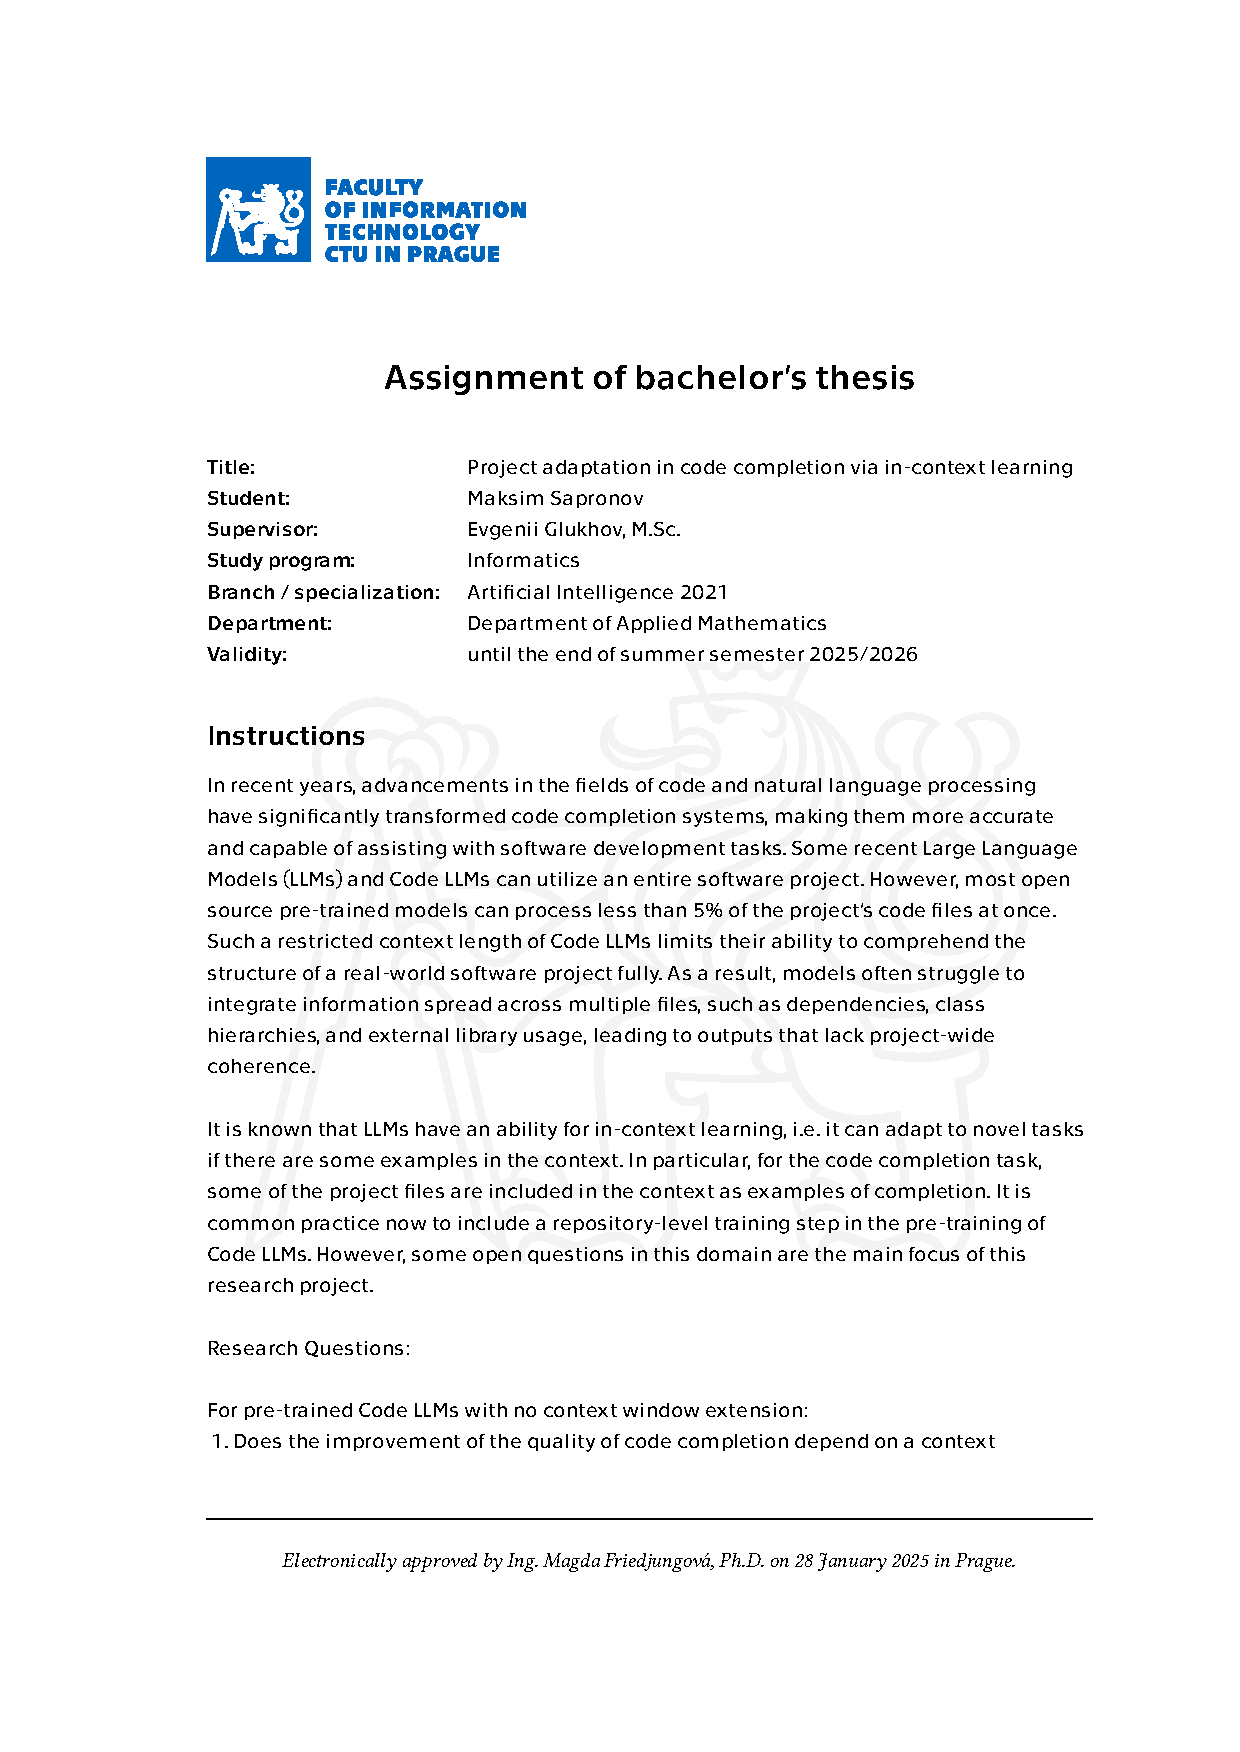
\includepdf[pages={1-}]{assignment.pdf}

\imprintpage
\stopTOCentries
%%%%%%%%%%%%%%%%%%%%%%
% list of other contents END
%%%%%%%%%%%%%%%%%%%%%%

% TODO: fill in the acknowledgment page
\begin{acknowledgmentpage}
	Thank you $\dots$
\end{acknowledgmentpage}

% TODO: choose one of approved texts of the declaration. DO NOT CREATE YOUR OWN. Find the approved texts at https://courses.fit.cvut.cz/SFE/download/index.html#_documents (document Declaration for FT in English)
\begin{declarationpage}
    Declaration content.
\end{declarationpage}

\printabstractpage

% TODO: decide whether to include the summary

\tableofcontents
%%%%%%%%%%%%%%%%%%%%%%
% list of other contents: figures, tables, code listings, algorithms, etc.
% add/remove commands accordingly
%%%%%%%%%%%%%%%%%%%%%%
\listoffigures % list of figures
\begingroup
\let\clearpage\relax
\listoftables % list of tables
\thectufitlistingscommand
\endgroup

% TODO: fill in the abbreviations (here is an irrelevant example)
\chapter{\thectufitabbreviationlabel}

\begin{tabular}{rl}
DFA & Deterministic Finite Automaton\\
FA & Finite Automaton\\
LPS & Labelled Prüfer Sequence\\
NFA & Nondeterministic Finite Automaton\\
NPS & Numbered Prüfer Sequence\\
XML & Extensible Markup Language\\
XPath & XML Path Language\\
XSLT & eXtensible Stylesheet Language Transformations\\
W3C & World Wide Web Consortium
\end{tabular}

\resumeTOCentries
\mainmatter\mainmatterinit
%%%%%%%%%%%%%%%%%%%
% THE THESIS
% MODIFY ANYTHING BELOW THIS LINE
%%%%%%%%%%%%%%%%%%%

\chapter*{Objectives of the Thesis}\addcontentsline{toc}{chapter}{Objectives of the Thesis}\markboth{Objectives of the Thesis}{Objectives of the Thesis}

The objectives of this thesis are divided into two parts, corresponding to the theoretical and practical aspects of the work.

The theoretical part aims to provide a comprehensive survey of the challenges associated with project adaptation in the context of full line code completion, focusing on the current capabilities and limitations of in-context learning and repository-level code completion methods. This part establishes the necessary background to understand the practical contributions of the thesis.

The practical part addresses several research questions concerning the impact of various context composition strategies on the quality of code completion, evaluated across three setups: a pre-trained Code Large Language Model (Code LLM), the same model fine-tuned with a specific context composition strategy, and the model after context window extension. To address these questions, the thesis implements a context composition framework for extracting relevant information from software repositories, as well as a fine-tuning pipeline for adapting Code LLMs to project-specific data. The outcomes characterize the role of context composition in enhancing code completion quality and provide insights into its integration within repository-level training procedures.

\chapter*{Introduction}\addcontentsline{toc}{chapter}{Introduction}\markboth{Introduction}{Introduction}

Software development plays a pivotal role in shaping the modern digital world. Assisting developers in writing code more efficiently has the potential to accelerate innovation across industries by reducing the cognitive and temporal overhead of programming. Over the decades, numerous tools have emerged to support developers, including high-level programming languages, integrated development environments (IDEs), version control systems, and, more recently, AI-powered code assistance. Tasks such as code completion, generation, refactoring, and bug localization are increasingly addressed using Large Language Models (LLMs), which have demonstrated strong capabilities in natural language and code understanding.

Code completion, in particular, benefits significantly from the in-context learning capabilities of LLMs — where the model leverages examples or relevant information provided in the input context to improve predictions without parameter updates. However, while LLMs have advanced in modeling local contexts, a critical limitation remains: their restricted ability to integrate and reason over information dispersed across large codebases. This includes understanding dependencies between files, class hierarchies, and interactions with external libraries — information that is often essential for generating coherent and accurate completions.

Despite the emergence of code-specific LLMs and efforts to incorporate repository-level context during training or inference, most pre-trained models still struggle to process more than a small fraction of a project's code files at once. As a result, they fall short in capturing project-wide structure, leading to incomplete or inaccurate predictions. Therefore, there is a need for continued research within the community developing such models to address these limitations. This thesis focuses on exploring how the composition and organization of contextual information influence the performance of code completion models, particularly in repository-level settings where code is distributed across multiple interdependent files. It investigates how context selection strategies and model adaptations can enhance the ability of pre-trained Code LLMs to generate coherent and accurate completions that reflect the structure and semantics of entire software projects.

% TODO: highlight the novelty of the work
% TODO: references?
% TODO: fill in the structure of the thesis here (w/ or w/o the example list)
% \begin{description}
    % \item[Chapter 1] Description of the first chapter.
    % \item[Chapter 2] Description of the second chapter.
% \end{description}

\chapter{Code Completion}\label{chap:code-completion}

The upcoming chapter provides a comprehensive examination of code completion. It begins with a definition of the task. The chapter then delves into the motivations for advancing code completion techniques, highlighting their impact on productivity and learning. A historical overview of the evolution of code completion methods is presented, tracing the transition from deterministic approaches to sophisticated learning-based systems. Finally, the chapter categorizes code completion based on various criteria.

\section{Task Definition}
% Relevant papers: bhoopchand2016, ginzberg2017, husein2025, izadi2024, wang2021, ciniselli2021, hindle2012, izadi2022, lu2021

Code completion, also called code suggestion or autocompletion, is a functionality within integrated development environments that enables developers to utilize an automated continuation of the code they are writing. Typically, it is invoked by a trigger model, which aims to anticipate the user's requirement for this functionality. The point of this invocation, whether it is referenced as temporal or spatial, is called a trigger point.

In this work, code completion is regarded as a task rather than a feature, as this perspective highlights the task-methodology relationship and emphasizes the technical aspects over marketing considerations. In addition, the term \textit{completion} is used as a shorthand throughout the text.

\section{Motivation}
% Relevant papers: peng2023, weber2024, bakal2025, takerngsaksiri2023, giagnorio2025

The task of code completion is a pivotal component of contemporary software development, offering substantial benefits that enhance both the productivity and efficiency of developers. This section elucidates the motivations for investigating this task and advancing existing solutions.

By reducing the amount of typing required, code completion allows developers to focus more on the logic and structure of their code rather than the syntax. Studies have shown that AI-powered code completion tools can significantly reduce task execution times, with some reporting up to a 55.8\% reduction in controlled experiments \parencite{peng2023}. These tools also significantly impact developer productivity by reducing the cognitive load associated with coding tasks, achieved through contextually relevant suggestions that streamline the coding process \parencite{weber2024}. Furthermore, the integration of AI in code completion tools has been linked to increased developer satisfaction and efficiency, as it allows developers to complete tasks more swiftly and with greater accuracy \parencite{bakal2025}.

For students and novice programmers, code completion tools serve as a valuable learning aid. They provide real-time feedback and suggestions, helping learners understand programming concepts and syntax more effectively. This educational aspect is highlighted in studies where students reported enhanced learning experiences and increased confidence in their coding abilities \parencite{takerngsaksiri2023}. Moreover, code completion tools provide accurate suggestions that help reduce typo errors and other common mistakes. This is particularly beneficial for new developers or those working with unfamiliar codebases, as it helps them adhere to coding standards and best practices.

Recent advancements in deep learning have enabled the personalization of code completion tools, allowing them to adapt to specific organizational or individual coding styles. This personalization not only improves the relevance of suggestions but also enhances the overall user experience, making these tools more effective and user-friendly \parencite{giagnorio2025}.

Due to the simple and atomic formulation of code completion, it possesses the important property of being fundamental to other AI-powered code assistance features. For instance, code generation can be viewed as a specific extension of code completion, and code editing is a sequence of code generations. This implies that most enhancements achieved through code completion research propagate further, adding new layers of improvements in the field.

In summary, code completion stands as a foundational and multifaceted tool within modern software development. Its benefits extend beyond mere convenience, offering measurable improvements in efficiency, learning, and code quality. As advancements in AI continue to refine its capabilities, code completion not only streamlines day-to-day programming tasks but also acts as a cornerstone for broader innovations in AI-assisted software engineering.

\section{Evolution of Methods}\label{sec:evolution-of-code-completion}
% Relevant papers: mandelin2005, hill2004, han2009, hindle2012, raychev2014, asaduzzaman2014, proksch2015, nguyen2015, bielik2016, ginzberg2017, karampatsis2019, liu2020, alon2019, svyatkovskiy2020, kim2021

\begin{sloppypar}
Approaches to code completion have evolved considerably over the past few decades, progressing from simple deterministic methods to sophisticated learning-based systems. This section highlights key developments in the history of code completion. The Related Work section of the~\citet{ciniselli2021} was mainly used to compile this valuable information.
\end{sloppypar}

In the early years, code completion methods primarily relied on rule-based approaches and static type information. These systems typically presented the user with a list of type-compatible methods or variables, often sorted alphabetically~\parencite{mandelin2005}. While straightforward to implement, these methods lacked contextual awareness and often produced lengthy suggestion lists that were cumbersome to navigate.

A significant advancement came with clone-based completion methods, where code fragments from existing repositories were identified and reused as completion suggestions \parencite{hill2004}. These approaches recognized that developers often write repetitive code patterns, but they were limited by the need for exact or near-exact matches in the code database.

The next major evolution occurred when researchers began applying statistical methods to code completion. \citet{han2009} introduced a novel approach that expanded abbreviated inputs into complete code tokens using Hidden Markov Models trained on example code. This represented an early step toward probabilistic code completion. \citet{hindle2012} demonstrated that software exhibits natural patterns that can be captured by statistical language models, laying the groundwork for treating code completion as a language modeling problem.

Building on this foundation, more sophisticated probabilistic models were developed. \citet{raychev2014} applied statistical language models specifically for code completion tasks, while \citet{bielik2016} introduced probabilistic higher order grammar (PHOG), which parameterized grammar production rules on a context obtained from executing functions learned from data. Bayesian networks were also explored by \citet{proksch2015}, who used additional context information beyond just the static type to generate completion suggestions.

Context-sensitivity became increasingly important as code completion systems matured. \citet{asaduzzaman2014} developed CSCC, which leveraged previous code examples to recommend method calls by considering the surrounding code context. This approach demonstrated how incorporating more contextual information affects the relevance of completion suggestions.

\begin{sloppypar}
The rise of deep learning brought another paradigm shift to code completion. Recurrent neural networks (RNNs), particularly long short-term memory (LSTM) networks, were applied to model the sequential nature of code. \citet{ginzberg2017} explored both standard LSTMs and attention-augmented networks for token-level code completion, establishing new capabilities in code prediction tasks.
\end{sloppypar}

Recent years have witnessed the adoption of even more powerful neural architectures. \citet{karampatsis2019} tackled the out-of-vocabulary problem in code completion using subword units with neural language models. \citet{liu2020} leveraged multi-task learning and pre-trained language models for code completion, while also incorporating type information to assist in identifier prediction.

The latest advancements utilize transformer-based architectures, which have proven effective in natural language processing (NLP). \citet{svyatkovskiy2020} introduced IntelliCode Compose, a general-purpose code completion tool that predicts sequences of code tokens using a transformer model. \citet{kim2021} enhanced transformer models by incorporating syntactic structure awareness through abstract syntax tree (AST)-based representations. These transformer architectures address limitations of previous sequence models by allowing attention to any part of the input context, rather than relying solely on sequential information. Furthermore, attention mechanisms enable transformers to consider relationships between distant parts of the code that have semantic connections, overcoming the long-range dependency challenges faced by RNN-based approaches.

Parallel to these developments, structural approaches that go beyond treating code as a mere sequence of tokens have gained prominence. \citet{alon2019} proposed a structural language modeling approach that leverages the strict syntax of programming languages to model code as a tree, capturing both syntactic and semantic relationships in the code. These structure-aware models offer an alternative to purely sequential approaches by explicitly modeling the hierarchical nature of source code.

The evolution of code completion methods reflects a general trend toward more contextually aware, semantically rich, and structurally informed models that capture the unique characteristics of source code compared to natural language. It also emphasizes the dominance of the probabilistic approaches over the deterministic ones.

\section{Taxonomy of Code Completion}
% Relevant papers: bhoopchand2016, ginzberg2017, husein2025, izadi2024, wang2021, ciniselli2021, hindle2012, izadi2022, lu2021

The concept of code completion lacks a strict definition within the field, as its interpretation has evolved with the various approaches employed to address it over time (see \sectionref{sec:evolution-of-code-completion} for more details). This section provides a comprehensive overview of the diverse characteristics of code completion and highlights the specific focus of this thesis.

To grasp the meaning of the subsequent text, it is crucial to understand the term \textit{token}, which refers to any subsequence of characters with a finite length.  % TODO: add a forward reference

\subsubsection*{Granularity}

Completion can be applied under the different degrees of granularity, which refers to the scope and detail of the produced code. At the most basic level, next-token completion involves predicting the subsequent token, such as a keyword, operator, or identifier. This level of granularity is useful for fine-grained suggestions that assist developers in writing code efficiently. Moving up in complexity, single line completion involves predicting the continuation of the given line of code based on the current context, which requires a broader understanding of the code's structure and logic. At the highest level, code block completion involves generating entire blocks of code, such as functions or classes, which necessitates a comprehensive understanding of the codebase and its architecture. This level of granularity is akin to code generation, where the model not only completes existing code but also creates new, coherent code structures. Each level of granularity serves different purposes and can be leveraged depending on the specific needs of the development task at hand.

For this work, single-line completion is selected because it presents a greater challenge for modern models compared to next-token prediction and serves as a fundamental baseline task for evaluating the performance of the proposed methods.

\subsubsection*{Context}

In the realm of code completion, a distinction is drawn between file-level and repository-level approaches, each characterized by its scope and contextual depth. File-level code completion operates within the confines of a single file, leveraging the immediate context such as local variable declarations, function definitions, and imports. This approach is effective for small, isolated scripts but is limited in its ability to capture the broader interactions present in larger projects. Conversely, repository-level code completion extends its reach to encompass the entire codebase, integrating information from multiple files and modules. This broader context is essential for understanding complex dependencies and interactions that span across the repository, enabling more accurate and contextually relevant code suggestions. The need for greater context in repository-level completion is driven by the intricate and interconnected nature of modern software systems, where a comprehensive understanding of the entire codebase is crucial for effective code completion.

Repository-level completion has been selected as the focus of this thesis because it offers a broader research landscape and addresses a significant need within the field.

\subsubsection*{Suffix Awareness}

The completion scenario can be categorized based on the directionality of the prediction relative to the trigger point. The left-to-right scenario involves generating code predictions using only the context preceding the trigger point, which is typical in traditional code completion systems. This approach is effective for straightforward code continuations but may lack the ability to consider the broader context. Conversely, the left-and-right scenario, also known as bidirectional completion, leverages both the preceding and succeeding context around the trigger point. This method allows for more informed predictions by considering the entire file, thus enhancing the accuracy and relevance of the suggestions.

Modern models for code completion employ the fill-in-the-middle (FIM) approach to gain suffix awareness capability. Although this thesis describes this method in \sectionref{sec:fill-in-the-middle}, it does not expand on it and instead focuses on the more fundamental left-to-right scenario. This choice is driven by the practical part of this work and its design constraints, which are motivated in \sectionref{sec:training}.

\subsubsection*{Line Start Availability}

Another criterion for categorizing completion systems is whether the initial portion of the target line has already been completed by the user. In practical applications, this scenario is quite common. However, for the purpose of model evaluation, it is more straightforward to assess the full line completion, where the initial part of the target line is not provided. This approach serves as a lower bound for assessing completion quality, as the ability to predict the entire line demonstrates a stronger capability.

Due to the aforementioned reasoning, the full line code completion is further considered throughout this thesis.

\subsubsection*{Programming Language Support}

The code completion systems can support either a single programming language (PL) or multiple languages simultaneously.

In the practical part of this thesis, multilingual models are employed with a focus on a single PL, specifically Python\footnote{\url{https://www.python.org/}}. This design choice is motivated by resource constraints.
\medskip

To finalize the terminology used in subsequent parts of this thesis regarding this task, the \textit{completion} refers to a full, single-line, repository-level code completion without suffix awareness.


\appendix\appendixinit

\chapter{Appendix}

\section{Supplementary Figures and Tables}

\begin{table}[htbp]
    \centering
    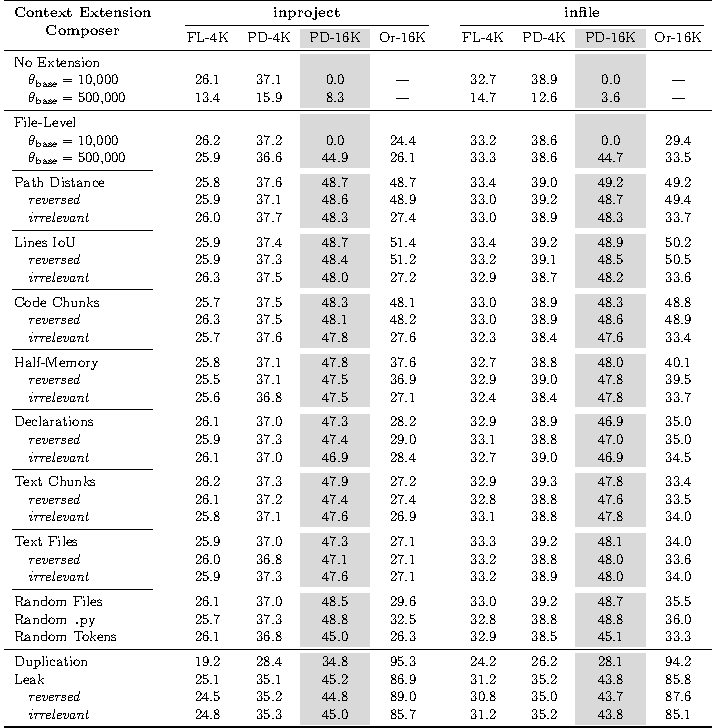
\includegraphics[width=\textwidth]{tables/rq-b.pdf}
    \caption{Extended table presenting the evaluation results for OpenCoder-1.5B-Base, which underwent the repository-level pre-training stage. A more detailed description of the evaluation setup is provided in Section~\ref{sec:evaluation}.}\label{tab:ocoder-extension-extended}
\end{table}

\begin{table}[htbp]
    \centering
    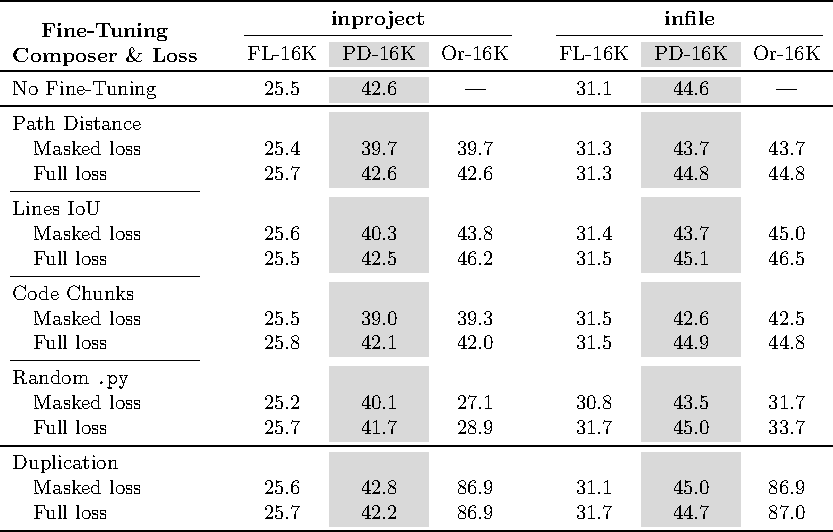
\includegraphics[width=\textwidth]{tables/rq-a2-gradient-masking.pdf}
    \caption{Exact Match scores for DeepSeek-Coder-Base 1.3B fine-tuned on composers generating inlier repository context for the completion file under two training setups: with and without gradient masking}\label{tab:dseek-gradient-masking}
\end{table}

\begin{table}[htbp]
    \centering
    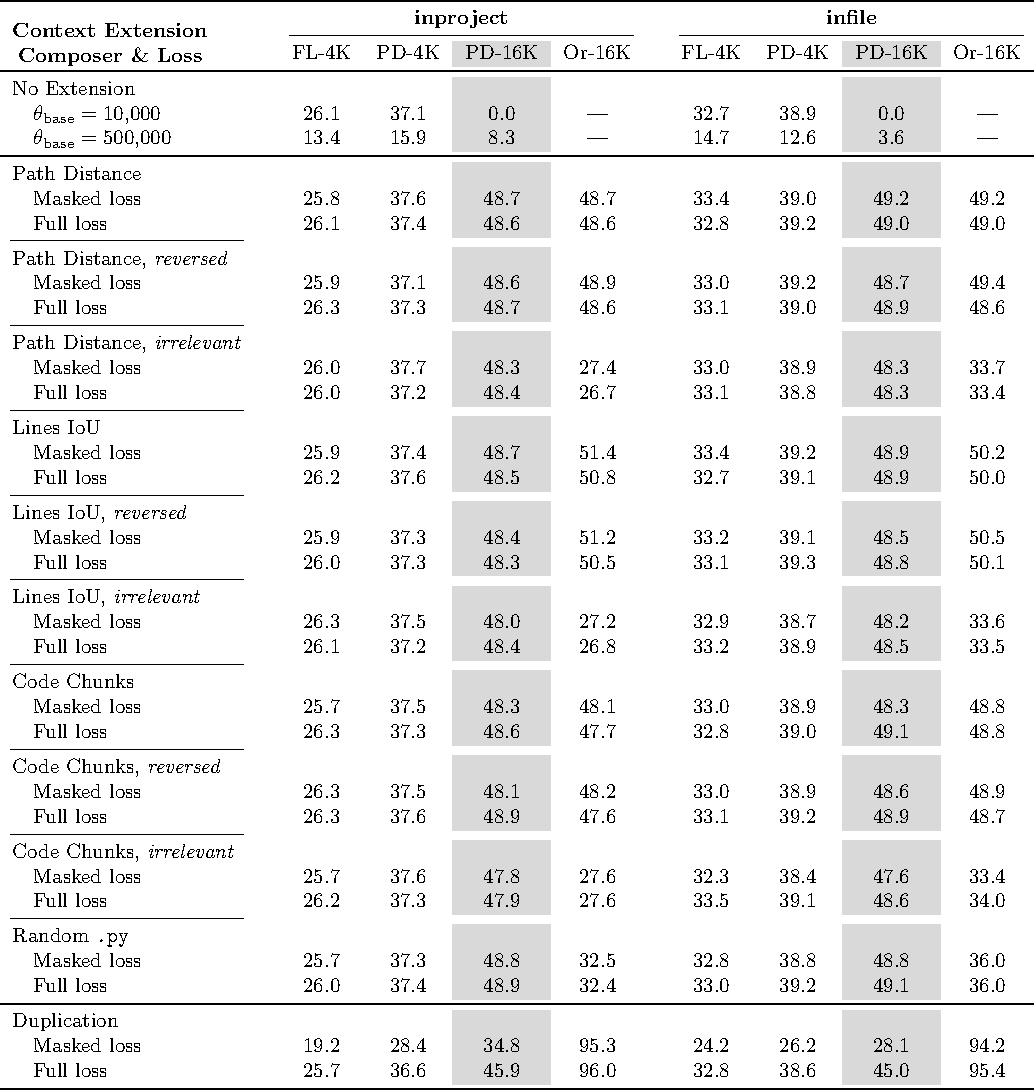
\includegraphics[width=\textwidth]{tables/rq-b-gradient-masking.pdf}
    \caption{Exact Match scores for repository-level pre-trained OpenCoder-1.5B-Base on composers generating inlier repository context for the completion file under two training setups: with and without gradient masking}\label{tab:ocoder-gradient-masking}
\end{table}

\begin{figure}[ht]
    \centering
    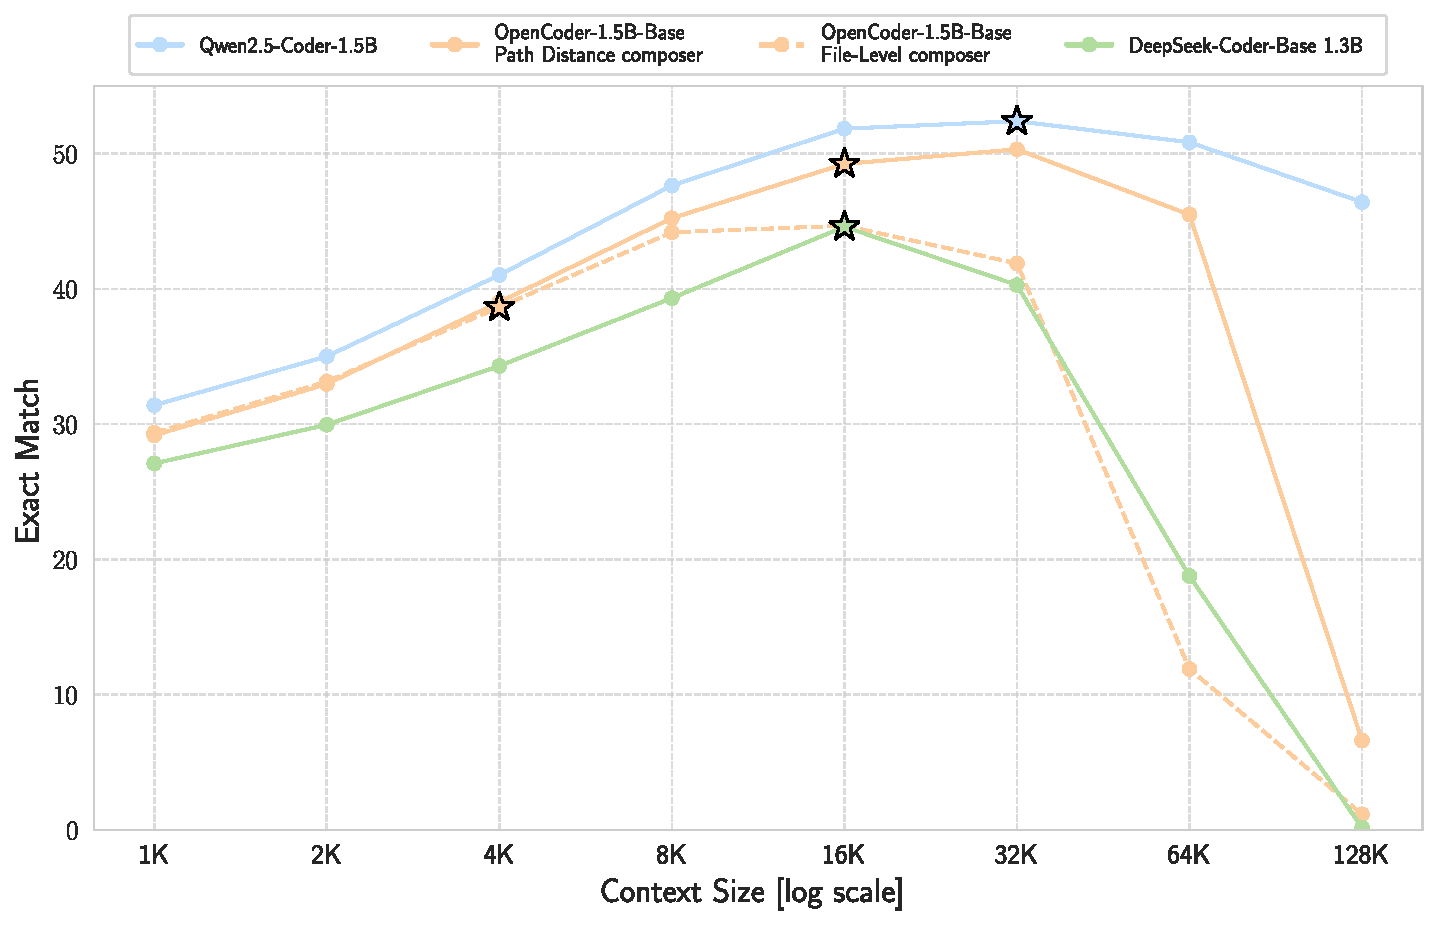
\includegraphics[width=\textwidth]{figures/beyond-training-window-infile.pdf}
    \caption{Evaluation of the performance scaling beyond the context extension window. The \textit{infile} line type from the LCA benchmark is selected for visualization; the corresponding Figure~\ref{fig:beyond-training-window-inproject} presents results for the \textit{inproject} category. ``1K'' refers to 1,024 tokens. The \raisebox{-0.3ex}{\FiveStarOpen} markers denote the context length used during repository-level pre-training stage.}\label{fig:beyond-training-window-infile}
\end{figure}
 % include `appendix.tex' from `text/' subdirectory

\backmatter

\printbibliography % print out the BibLaTeX-generated bibliography list

\chapter{Contents of the attachment}

Not ready.

	% TODO: fill in the contents of the attachment (irrelevant example is provided)
	% \dirtree{%
	% 	.1 /.
	% 	.2 readme.txt\DTcomment{short description of the media}.
	% 	.2 exe\DTcomment{directory with the executable form of the implementation}.
	% 	.2 src.
	% 	.3 impl\DTcomment{source codes of the implementation}.
	% 		.3 thesis\DTcomment{zdrojová forma práce ve formátu \LaTeX{}}.
	% 		.2 text\DTcomment{text práce}.
	% 		.3 thesis.pdf\DTcomment{text práce ve formátu PDF}.
	% }
 % include `medium.tex' from `text/' subdirectory

\end{document}
